% Every perturbation position of models/positions.py VIT_POSITIONS, drawn on 1
% ViT-B/16 encoder block, with the 2 named placements highlighted. Compiled by
% notebooks/figures/render.py.
\documentclass[tikz,border=6pt]{standalone}
\usepackage[T1]{fontenc}
\usepackage{lmodern}
\usetikzlibrary{arrows.meta,positioning,fit,backgrounds,calc}

\definecolor{tm}{HTML}{009E73}
\definecolor{rd}{HTML}{D55E00}
\definecolor{other}{HTML}{0072B2}
\definecolor{boxfill}{HTML}{F2F2F2}

\tikzset{
  op/.style={draw, rounded corners=2pt, fill=boxfill, minimum height=8mm,
    minimum width=13mm, font=\small\sffamily, align=center},
  add/.style={draw, circle, inner sep=0pt, minimum size=5mm, font=\small},
  flow/.style={-{Stealth[length=2mm]}, thick},
  probe/.style={circle, fill=other, inner sep=0pt, minimum size=2.4mm},
  probetm/.style={circle, fill=tm, inner sep=0pt, minimum size=3.2mm},
  proberd/.style={circle, fill=rd, inner sep=0pt, minimum size=3.2mm},
  lab/.style={font=\scriptsize\ttfamily, align=center, text=other},
  labtm/.style={font=\scriptsize\ttfamily\bfseries, align=center, text=tm},
  labrd/.style={font=\scriptsize\ttfamily\bfseries, align=center, text=rd},
}

\begin{document}
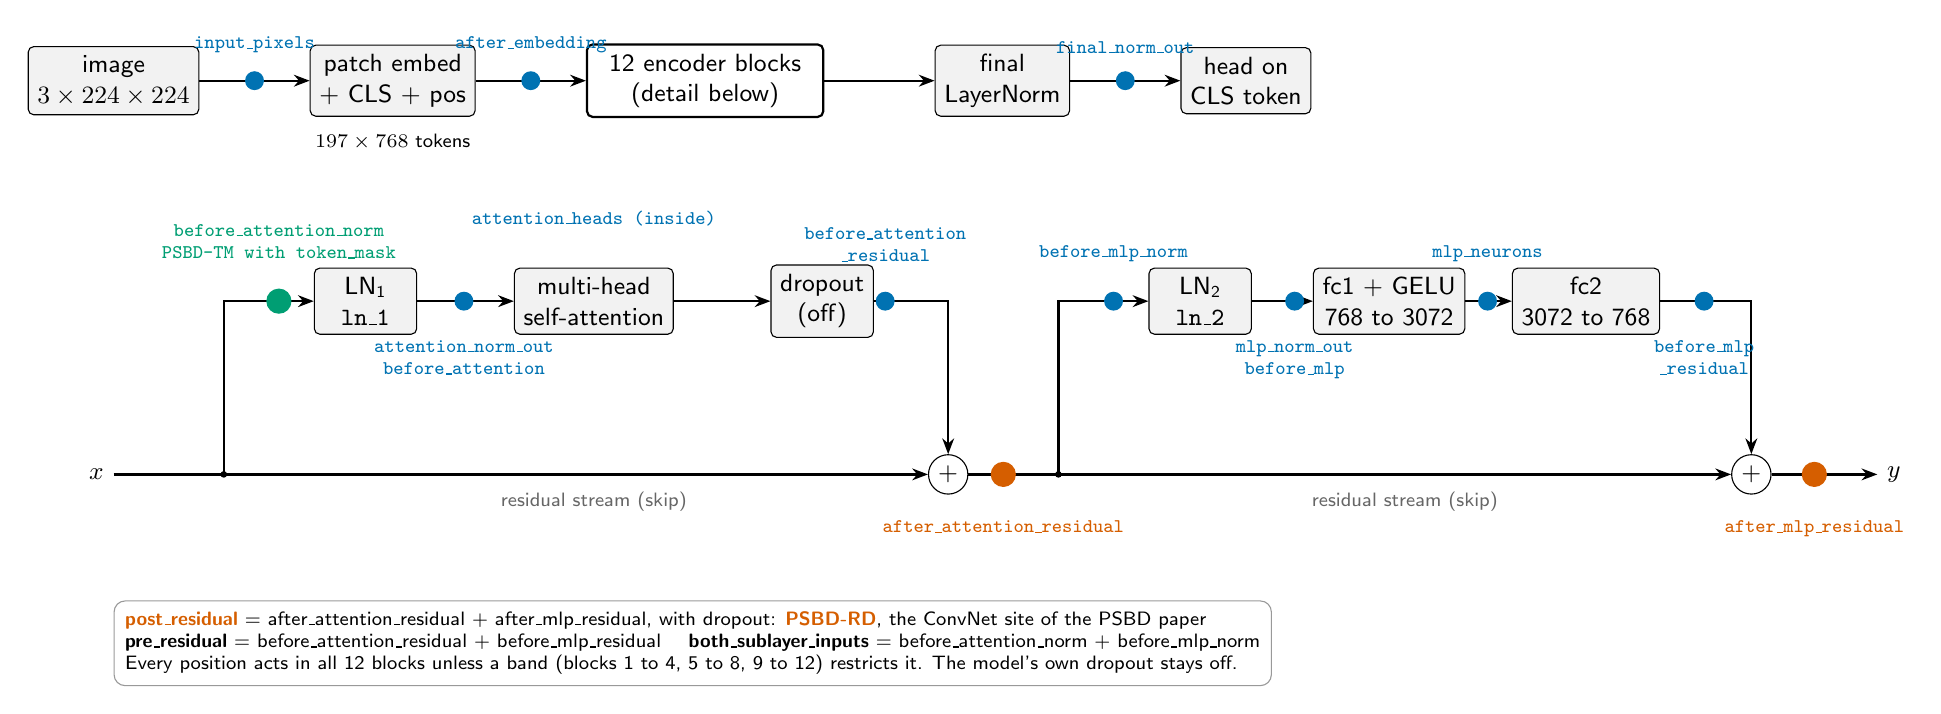
\begin{tikzpicture}

% The model level: the image enters, is embedded, crosses 12 blocks and is read
% off the class token.
\node[op] (img) at (0, 5.0) {image\\$3\times224\times224$};
\node[op, right=14mm of img] (embed) {patch embed\\+ CLS + pos};
\node[op, right=14mm of embed, minimum width=30mm, fill=white, thick] (blocks)
  {12 encoder blocks\\(detail below)};
\node[op, right=14mm of blocks] (fln) {final\\LayerNorm};
\node[op, right=14mm of fln] (head) {head on\\CLS token};
\draw[flow] (img) -- (embed);
\draw[flow] (embed) -- (blocks);
\draw[flow] (blocks) -- (fln);
\draw[flow] (fln) -- (head);

\node[probe] (p_in) at ($(img.east)!0.5!(embed.west)$) {};
\node[lab, above=1mm of p_in] {input\_pixels};
\node[probe] (p_emb) at ($(embed.east)!0.5!(blocks.west)$) {};
\node[lab, above=1mm of p_emb] {after\_embedding};
\node[probe] (p_fln) at ($(fln.east)!0.5!(head.west)$) {};
\node[lab, above=1mm of p_fln] {final\_norm\_out};
\node[font=\scriptsize\sffamily, below=1mm of embed] {$197\times768$ tokens};

% The block, pre-norm form: x' = x + Dropout(MSA(LN1(x))), y = x' + MLP(LN2(x')).
\coordinate (in) at (0, 0);
\coordinate (split1) at (1.4, 0);
\node[op] (ln1) at (3.2, 2.2) {LN\textsubscript{1}\\\texttt{ln\_1}};
\node[op, minimum width=20mm] (msa) at (6.1, 2.2) {multi-head\\self-attention};
\node[op] (drop1) at (9.0, 2.2) {dropout\\(off)};
\node[add] (add1) at (10.6, 0) {$+$};
\coordinate (split2) at (12.0, 0);
\node[op] (ln2) at (13.8, 2.2) {LN\textsubscript{2}\\\texttt{ln\_2}};
\node[op] (fc1) at (16.2, 2.2) {fc1 + GELU\\768 to 3072};
\node[op] (fc2) at (18.7, 2.2) {fc2\\3072 to 768};
\node[add] (add2) at (20.8, 0) {$+$};
\coordinate (out) at (22.4, 0);

\draw[flow] (in) -- (add1);
\draw[flow] (split1) |- (ln1);
\draw[flow] (ln1) -- (msa);
\draw[flow] (msa) -- (drop1);
\draw[flow] (drop1) -| (add1);
\draw[flow] (add1) -- (add2);
\draw[flow] (split2) |- (ln2);
\draw[flow] (ln2) -- (fc1);
\draw[flow] (fc1) -- (fc2);
\draw[flow] (fc2) -| (add2);
\draw[flow] (add2) -- (out);
\fill (split1) circle (1.2pt);
\fill (split2) circle (1.2pt);

\node[font=\small\sffamily, anchor=east] at (in) {$x$};
\node[font=\small\sffamily, anchor=west] at (out) {$y$};
\node[font=\scriptsize\sffamily, text=black!60] at (6.1, -0.35) {residual stream (skip)};
\node[font=\scriptsize\sffamily, text=black!60] at (16.4, -0.35) {residual stream (skip)};

% Branch-side positions: a pre-hook or post-hook on 1 module, the skip untouched.
\node[probetm] (p_ban) at (2.1, 2.2) {};
\node[labtm, above=2.5mm of p_ban] {before\_attention\_norm\\PSBD-TM with token\_mask};
\node[probe] (p_ano) at (4.45, 2.2) {};
\node[lab, below=2.5mm of p_ano] {attention\_norm\_out\\before\_attention};
\node[font=\scriptsize\ttfamily, text=other, align=center] at (6.1, 3.25) {attention\_heads (inside)};
\node[probe] (p_bar) at (9.8, 2.2) {};
\node[lab, above=2.5mm of p_bar] {before\_attention\\\_residual};
\node[probe] (p_bmn) at (12.7, 2.2) {};
\node[lab, above=2.5mm of p_bmn] {before\_mlp\_norm};
\node[probe] (p_mno) at (15.0, 2.2) {};
\node[lab, below=2.5mm of p_mno] {mlp\_norm\_out\\before\_mlp};
\node[probe] (p_neu) at (17.45, 2.2) {};
\node[lab, above=2.5mm of p_neu] {mlp\_neurons};
\node[probe] (p_bmr) at (20.2, 2.2) {};
\node[lab, below=2.5mm of p_bmr] {before\_mlp\\\_residual};

% Stream-side positions: the tensor both the next branch and the skip read.
\node[proberd] (p_aar) at (11.3, 0) {};
\node[labrd, below=3mm of p_aar] {after\_attention\_residual};
\node[proberd] (p_amr) at (21.6, 0) {};
\node[labrd, below=3mm of p_amr] {after\_mlp\_residual};

% The composite placements of models.positions.DROPOUT_CONFIGS.
\node[draw=black!40, rounded corners, font=\scriptsize\sffamily, align=left,
  anchor=north west, inner sep=4pt] at (0, -1.6) {%
  \textcolor{rd}{\textbf{post\_residual}} = after\_attention\_residual + after\_mlp\_residual, with dropout: \textcolor{rd}{\textbf{PSBD-RD}}, the ConvNet site of the PSBD paper\\
  \textbf{pre\_residual} = before\_attention\_residual + before\_mlp\_residual \quad
  \textbf{both\_sublayer\_inputs} = before\_attention\_norm + before\_mlp\_norm\\
  Every position acts in all 12 blocks unless a band (blocks 1 to 4, 5 to 8, 9 to 12) restricts it. The model's own dropout stays off.};

\end{tikzpicture}
\end{document}
